Para realizar la pantalla de supervisión, control y adquisición de datos operador se utilizó el software iFix perteneciente al grupo \textit{General Electric}.

El sistema SCADA creado (Figura \ref{fig:scada1}) se dividió en las siguientes secciones:
\begin{itemize}
	\item Esquemático del circuito hidráulico físico con las variables de presión y caudal en tiempo real.
	\item Valores de funcionamiento del motor obtenidos por el variador de velocidad.
	\item Alarmero, dónde se observa de forma visual valores críticos alcanzados en el sistema.
	\item Indicador de modo de funcionamiento físico o remoto.
	\item Modo de control a lazo abierto o lazo cerrado.
	\subitem Para el modo de lazo cerrado se creó una ventana individual para cada sistema de presión y caudal.
	\item Pantalla para observar gráficos en tiempo real dónde se divide según la variable a observar, con botones para abrir el control PID del sistema.
	\item Pantalla donde se observa datos históricos y se puede generar un archivo \textit{.txt} con la información de la variable elegida en un determinado período de tiempo.
\end{itemize} 

\begin{figure}[htb]
	\centering
	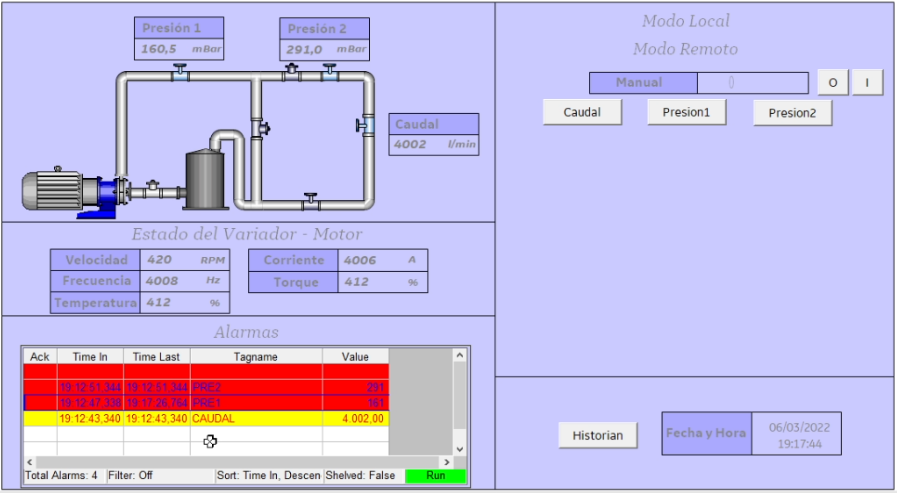
\includegraphics[width=0.9\linewidth]{scada1.png}
	\captionof{figure}{Pantalla SCADA}
	\label{fig:scada1}
\end{figure}


\subsubsection{Configuración driver Modbus}
Para realizar la configuración de cada ícono de la pantalla SCADA con su respectiva variable, se debió crear un MBE Driver (Figura \ref{fig:mbe}) dónde se estipula la dirección IP y el mapa de memoria con sus respectivas secciones que luego serán utilizadas por el DataBase (Figura \ref{fig:database}). 

Una vez creado el MBE Driver se debe generar la tabla \textit{DataBase} en dónde estará el nombre, dirección IP, tipo de elemento, descripción, alarma asociada, entre otros puntos de cada elemento.

\begin{figure}[h!]
	\centering
	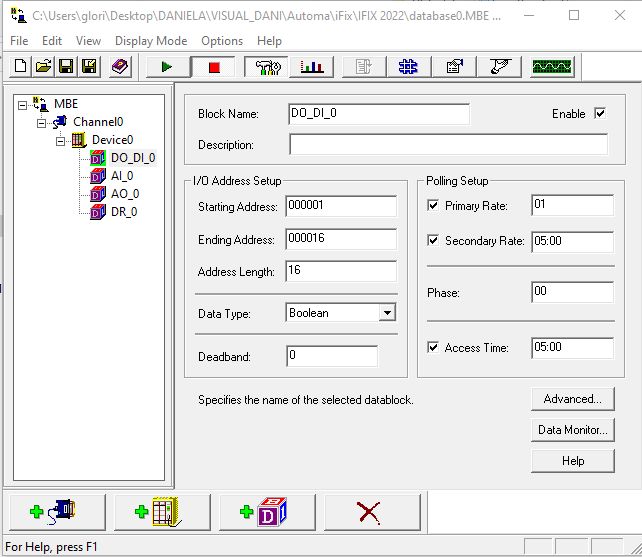
\includegraphics[width=0.8\linewidth]{mbe.png}
	\captionof{figure}{Configuración MBE}
	\label{fig:mbe}
\end{figure}
\begin{figure}[h!]
	\centering
	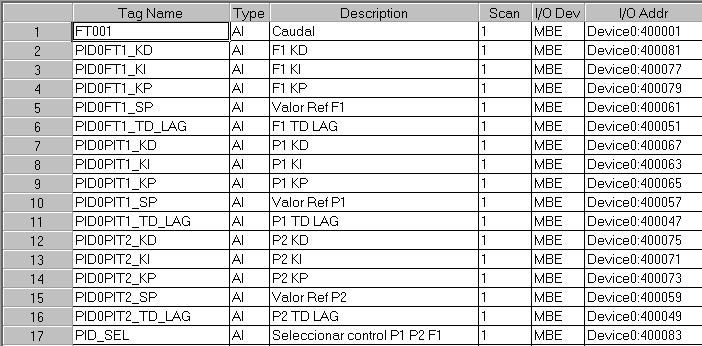
\includegraphics[width=0.8\linewidth]{database.png}
	\captionof{figure}{Database con MBE}
	\label{fig:database}
\end{figure}


\paragraph{Pruebas mediante ModSim}
Para realizar pruebas intermedias antes de unir SCADA con el programa del PLC se utilizó el software \textit{ModSim}, dónde se generó los distintos mapas de memoria utilizados para modificar variables y observar el correcto funcionamiento de distintos elementos en el SCADA (Figura \ref{fig:modsim1}).

\begin{figure}[h!]
	\centering
	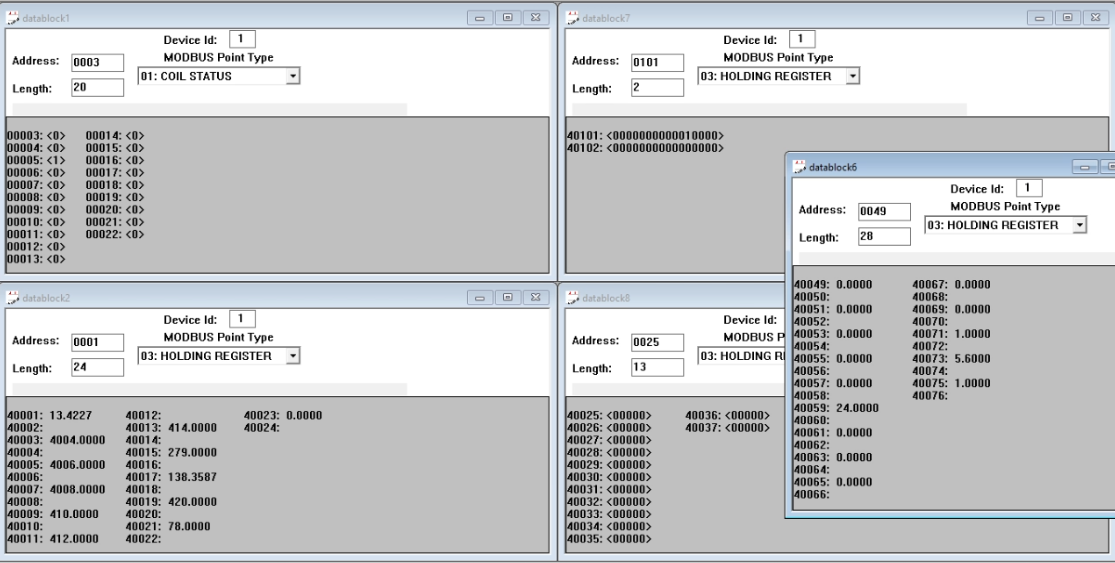
\includegraphics[width=0.7\linewidth]{modsim1.png}
	\captionof{figure}{ModSim}
	\label{fig:modsim1}
\end{figure}





\subsubsection{Alarmas}
Dentro de la pantalla principal es posible observar el alarmero. El la Tabla {\ref{c2_tabla_segento_tcp} se observa el diagrama causa efecto de cada alarma.  Por ejemplo, si la temperatura del motor es 50 °C, la alarma se activará informando alta temperatura, y si la temperatura llega a 70 °C, el variador de velocidad hará que el motor se detenga para que no se produzca un daño al bobinado.

	\begin{table}[h!]
	\centering
	\rotatebox{90}{		
		\resizebox{21cm}{!} {
			
			\begin{tabular}{|l|l|l|l|l|l|l|l|l|l|l|l|l|l|l|l|l|} 
				\hline
				\multicolumn{1}{|c|}{\multirow{2}{*}{\begin{tabular}[c]{@{}c@{}}\textbf{TAG}\\\textbf{INSTRUMENTO}\end{tabular}}} & \multicolumn{1}{c|}{\multirow{2}{*}{\textbf{SERVICIO}}} & \multicolumn{1}{c|}{\multirow{2}{*}{\textbf{UNIDADES}}} & \multicolumn{2}{c|}{\textbf{RANGO}}                                                                                               & \multicolumn{4}{c|}{\textbf{ALARMAS}}                                                                                                                                                                                                                                   & \multicolumn{5}{c|}{\textbf{ENCLAVAMIENTO}}                                                                                                                                                                                                                                                                                                 & \multicolumn{1}{c|}{\textbf{EFECTO}}                            & \multicolumn{1}{c|}{\multirow{2}{*}{\begin{tabular}[c]{@{}c@{}}\textbf{PROPOSITO DE }\\\textbf{ALARMA}\end{tabular}}} & \multicolumn{1}{c|}{\multirow{2}{*}{\begin{tabular}[c]{@{}c@{}}\textbf{CONSECUENCIA DE LA}\\\textbf{NO ACCION}\end{tabular}}}  \\ 
				\cline{4-15}
				\multicolumn{1}{|c|}{}                                                                                            & \multicolumn{1}{c|}{}                                   & \multicolumn{1}{c|}{}                                   & \multicolumn{1}{c|}{\begin{sideways}\textbf{MIN}\end{sideways}} & \multicolumn{1}{c|}{\begin{sideways}\textbf{MAX}\end{sideways}} & \multicolumn{1}{c|}{\begin{sideways}\textbf{HI-HI}\end{sideways}} & \multicolumn{1}{c|}{\begin{sideways}\textbf{HI}\end{sideways}} & \multicolumn{1}{c|}{\begin{sideways}\textbf{LO}\end{sideways}} & \multicolumn{1}{c|}{\begin{sideways}\textbf{LO-LO}\end{sideways}} & \multicolumn{1}{c|}{\begin{sideways}\textbf{DELAY}\end{sideways}} & \multicolumn{1}{c|}{\begin{sideways}\textbf{HI-HI}\end{sideways}} & \multicolumn{1}{c|}{\begin{sideways}\textbf{HI}\end{sideways}} & \multicolumn{1}{c|}{\begin{sideways}\textbf{LO}\end{sideways}} & \multicolumn{1}{c|}{\begin{sideways}\textbf{LO-LO}\end{sideways}} & \multicolumn{1}{c|}{\begin{sideways}\textbf{VSD}\end{sideways}} & \multicolumn{1}{c|}{}                                                                                                 & \multicolumn{1}{c|}{}                                                                                                          \\ 
				\hline
				\textbf{TE001}                                                                                                    & Temperatura                                             & °C                                                      &                                                                 &                                                                 &                                                                   &                                                                & 50                                                             &                                                                   &                                                                   &                                                                   &                                                                &                                                                &                                                                   &                                                                 & \begin{tabular}[c]{@{}l@{}}Informar alta temperatura \\del motor\end{tabular}                                         &                                                                                                                                \\ 
				\hline
				\textbf{TE001}                                                                                                    & Temperatura                                             & °C                                                      &                                                                 &                                                                 & 70                                                                &                                                                &                                                                &                                                                   &                                                                   & 70                                                                &                                                                &                                                                &                                                                   & P                                                               & \begin{tabular}[c]{@{}l@{}}Informar muy alta temperatura \\del motor\end{tabular}                                     & Daño al bobinado                                                                                                               \\ 
				\hline
				\textbf{PIT01}                                                                                                   & Presión                                                 & mbar                                                    & -1000                                                           & 4000                                                            & 700                                                               &                                                                &                                                                &                                                                   &                                                                   & 700                                                               &                                                                &                                                                &                                                                   & P                                                               & \begin{tabular}[c]{@{}l@{}}Informar alta presión \\en cañería\end{tabular}                                            & Daño a bomba                                                                                                                   \\ 
				\hline
				\textbf{PIT01}                                                                                                   & Presión                                                 & mbar                                                    &                                                                 &                                                                 &                                                                   &                                                                &                                                                &                                                                   &                                                                   &                                                                   &                                                                &                                                                & -1                                                                & P                                                               & Informar desconexión PIT01                                                                                           &                                                                                                                                \\ 
				\hline
				\textbf{PIT02}                                                                                                   & Presión                                                 & mbar                                                    & -1000                                                           & 4000                                                            &                                                                   &                                                                &                                                                &                                                                   &                                                                   &                                                                   &                                                                &                                                                & -1                                                                & P                                                               & Informar desconexión PIT02                                                                                           &                                                                                                                                \\ 
				\hline
				\textbf{FT01}                                                                                                    & Caudal                                                  & l/min                                                   & 0                                                               & 60                                                              &                                                                   &                                                                & 0.5                                                            &                                                                   & 30s                                                               &                                                                   &                                                                & 0.5                                                            &                                                                   & P                                                               & Informar bajo flujo                                                                                                   & Daño a bomba                                                                                                                   \\ 
				\hline
				\textbf{VSD\_SC001}                                                                                               & Velocidad                                               & rpm                                                     & 0                                                               & 3600                                                            & 200                                                               &                                                                &                                                                &                                                                   &                                                                   & 200                                                               &                                                                &                                                                &                                                                   & P                                                               & Informar baja velocidad                                                                                               & Daño a motor                                                                                                                   \\
				\hline
			\end{tabular}
			
			
		}
	}
	\caption{Causa- Efecto de las alarmas}
	\label{c2_tabla_segento_tcp}
	
\end{table}




\subsubsection{Paradas por bloqueo}
El banco de pruebas está preparado para detener el motor si ocurriese alguna anomalía y mostrar la falla en la pantalla SCADA en la parte inferior derecha. Se programó para que reconozca los siguientes errores en el sistema: 

\begin{itemize}
	\item \textit{Alta presión}
	\item \textit{Bajo caudal}
	\item \textit{Sensor de presión desconectado}
	\item \textit{Temperatura de motor alta}
	\item \textit{VSD sin comunicación}
\end{itemize}



\subsubsection{Datos históricos}
Para interpretar datos históricos se puede por dos métodos, uno es generar un archivo .txt y el otro es de forma gráfica. 
Se generó una pantalla SCADA prediseñada de iFix dónde al conectar con el servidor Historian, busca los datos históricos de la variable elegida y guarda un archivo .txt con el horario y valores. Se puede elegir más de una variable, pero se debe tener en cuenta que no se generan columnas nuevas sinó que generará en el mismo archivos más filas (Figura \ref{fig:scada33}.a).

Otra de las opciones es observar datos históricos en un gráfico de tiempo, estas variables están preestablecidas y son las presiones y el caudal con sus respectivos valores de referencias (Figura \ref{fig:scada33}.b).

\begin{figure}[htbp]
	\centering
	\subfigure[Pantalla datos históricos]{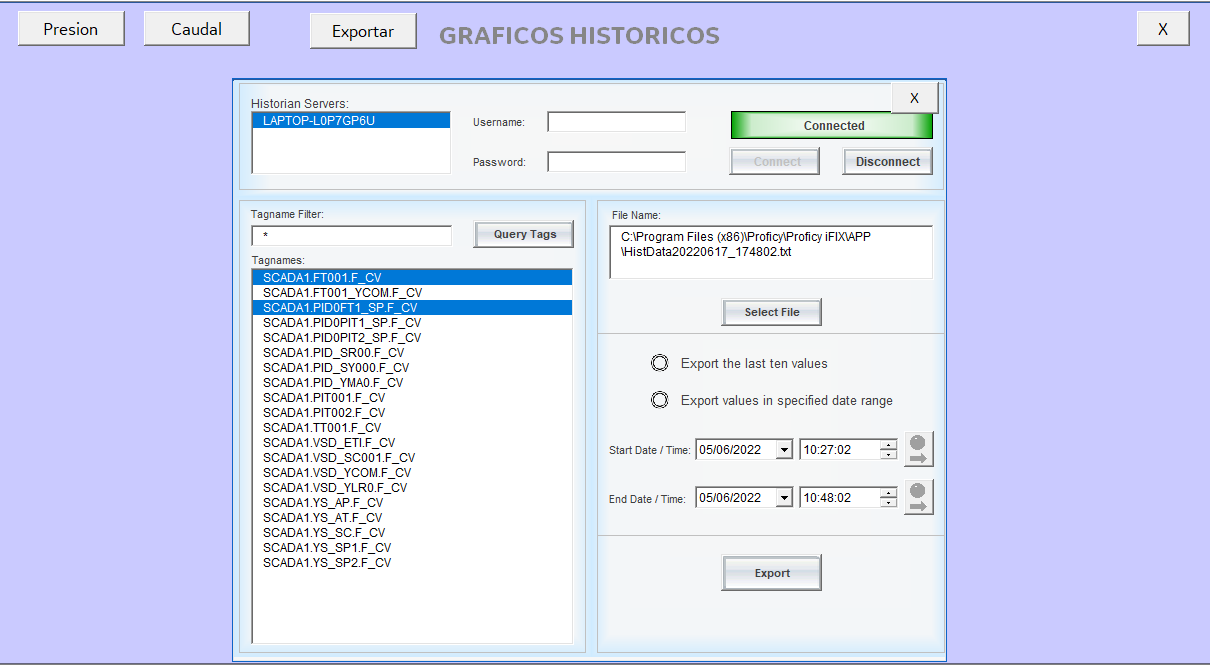
\includegraphics[width=1\linewidth]{scada33.png}}
	\subfigure[Guardar datos históricos]{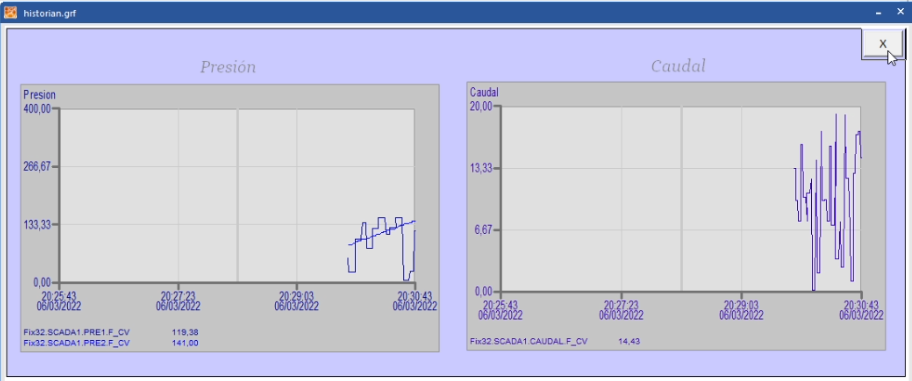
\includegraphics[width=1\linewidth]{scada3.png}}
	\caption{Datos históricos} \label{fig:scada33}
\end{figure}


